\section{Experiments}
\label{section:experiments}
\begin{table}
\begin{center}
    \begin{tabular}{cccccccc}
    \toprule
    \textbf{\#} & \textbf{S} &  & \textbf{M} & & \textbf{L} & & \textbf{XL} \\
    \midrule
    \textbf{Conv. Layers}      & 20 & & 30 & & 90 & & 120 \\
    \textbf{Channels}  &45 & & 60 & & 60 & & 70 \\ 
    \textbf{Lin. Layers}        &7 & & 10 & & 15 & & 15 \\
    \textbf{Lin. Features} & 2048 & & 2048 & & 4096 & & 4096 \\
    \bottomrule
    \end{tabular}%

\end{center}
\caption{\label{table:model-desc}
Architectures description for our Convex Potential Layers (CPL) neural networks with different capacities. We vary the number of Convolutional Convex Potential Layers, the number of Linear Convex Potential Layers, the number of channels in the convolutional layers and the width of fully
connected layers. In the paper, they will be reported respectively as CPL-S, CPL-M, CPL-L and CPL-XL.}
\end{table}

To evaluate our new $1$-Lipschitz Convex Potential Layers, we carry out an extensive set of experiments. In this section, we first describe  the details of our experimental setup. We then recall  the concurrent approaches that build $1$-Lipschitz Neural Networks and stress their limitations. Our experimental results are finally summarized in ection~\ref{sec:setting-xp}. By computing the certified and empirical adversarial  accuracy of our networks on CIFAR10 and CIFAR100 classification tasks~\citep{krizhevsky2009learning}, we show that our architecture is competitive with state-of-the-art methods (Sections~\ref{sec:results}). In Appendix~\ref{app:xp-supp}, we also study the influence of some hyperparameters and demonstrate the stability and the scalability of our approach by training very deep neural networks up to 1000 layers without normalization tricks or gradient clipping.










\subsection{Training and Architectural Details}
\label{sec:setting-xp}

We demonstrate the effectiveness of our approach on a classification task with CIFAR10 and CIFAR100 datasets~\citep{krizhevsky2009learning}. We use a similar training configuration to the one proposed in~\citep{trockman2021orthogonalizing}
We trained our networks with a batch size of $256$ over $200$ epochs.
We use standard data augmentation (\ie, random cropping and flipping), a learning rate of $0.001$ with Adam optimizer \citep{diederik2014adam} without weight decay and a piecewise triangular learning rate scheduler. We used a margin parameter in the loss set to $0.7$.

As other usual convolutional neural networks, we first stack few Convolutional CPLs and then stack some Linear CPLs for classification tasks. To validate the performance  and the scalability of our layers,  we will evaluate four different variations of different hyperparameters as described in Table~\ref{table:model-desc}, respectively named CPL-S, CPL-M, CPL-L and CPL-XL, ranked according to the number of parameters they have. In all our experiments, we made $3$ independent trainings to evaluate accurately the models. All reported results are the average of these $3$ runs.

\subsection{Concurrent Approaches} We compare our networks with SOC~\citep{skew2021sahil} and Cayley~\cite{trockman2021orthogonalizing} networks which are to our knowledge the best performing approaches for deterministic $1$-Lipschitz Neural Networks. Since our layers are fundamentally different from these ones, we cannot compare with the same architectures. We reproduced SOC results for with $10$ and $20$ layers, that we call respectively SOC-$10$ and SOC-$20$ in the same training setting, \emph{i.e.} normalized inputs, cross entropy loss, SGD optimizer with learning rate $0.1$ and multi-step learning rate scheduler. For Cayley layers networks, we reproduced their best reported model, \emph{i.e.} KWLarge with width factor of $3$. 

The work of~\citet{singla2021householder} propose three methods to improve certifiable accuracies from SOC layers: a new HouseHolder activation function (HH),  last layer normalization (LLN), and certificate regularization (CR). The code associated with this paper is not open-sourced yet, so we just reported the results from their paper in ours results (Tables~\ref{table:c10-comp} and~\ref{table:c100-comp}) under the name SOC+. We were being able to implement the LLN method in all models. This method largely improve the result of all methods on CIFAR100, so we used it for all networks we compared on CIFAR100 (ours and concurrent approaches).


\begin{table*}[tb]
  \centering
  \sisetup{%
    table-align-uncertainty=true,
    separate-uncertainty=true,
    detect-weight=true,
    detect-inline-weight=math
  }
  \begin{tabular}
  {
    l
    S[table-format=2.2]
    S[table-format=2.2]
    S[table-format=2.2]
    S[table-format=2.2]
    S[table-format=2.2]
  }
  \toprule
    & \multicolumn{1}{c}{\textbf{Clean Accuracy}} & \multicolumn{3}{c}{\textbf{Provable Accuracy ($\varepsilon $)}} &  \multicolumn{1}{c}{\textbf{Time per epoch (s)}} 
    \\
    \cmidrule{3-5}
    & \multicolumn{1}{c}{ } & \multicolumn{1}{c}{36/255} & \multicolumn{1}{c}{72/255} &  \multicolumn{1}{c}{108/255} & \multicolumn{1}{c}{\textbf{}} 
    \\
  \midrule
    \textbf{CPL-S} & 75.6  & 62.3  & 46.9  & 32.2  & 21.9 \\
  \textbf{CPL-M} & 76.8  & 63.3  & 47.5  & 32.5  & 40.0 \\
  \textbf{CPL-L} & 77.7  & 63.9 & 48.1 & 32.9  & 93.4 \\
  \textbf{CPL-XL} & 78.5  & 64.4  & 48.0  & 33.0 & 163 \\
  \midrule
  \textbf{Cayley (KW3)} & 74.6  & 61.4  & 46.4  & 32.1  & 30.8\\
    \midrule

  \textbf{SOC-10} & 77.6  & 62.0  & 45.0  & 29.5  & 33.4 \\
  \textbf{SOC-20} & 78.0  & 62.7 & 46.0  & 30.3  &52.2\\
  \midrule
    \textbf{SOC+-10} & 76.2 &62.6 & 47.7 & 34.2& N/A\\
  \textbf{SOC+-20} & 76.3&62.6& 48.7& 36.0& N/A \\

  \bottomrule
  \end{tabular}%
  \caption{Results on the CIFAR10 dataset on standard and  provably certifiable accuracies for different values of perturbations $\varepsilon$ on CPL (ours), SOC and Cayley models. The average time per epoch in seconds is also reported in the last column. None of these networks uses Last Layer Normalization.}
  \label{table:c10-comp}%
\end{table*}%

\begin{table*}[tb]
  \centering
  \sisetup{%
    table-align-uncertainty=true,
    separate-uncertainty=true,
    detect-weight=true,
    detect-inline-weight=math
  }
  \begin{tabular}
  {
    l
    S[table-format=2.2]
    S[table-format=2.2]
    S[table-format=2.2]
    S[table-format=2.2]
    S[table-format=2.2]
  }
  \toprule
    & \multicolumn{1}{c}{\textbf{Clean Accuracy}} & \multicolumn{3}{c}{\textbf{Provable Accuracy ($\varepsilon $)}} &  \multicolumn{1}{c}{\textbf{Time per epoch (s)}} 
    \\
    \cmidrule{3-5}
    & \multicolumn{1}{c}{ } & \multicolumn{1}{c}{36/255} & \multicolumn{1}{c}{72/255} &  \multicolumn{1}{c}{108/255} & \multicolumn{1}{c}{\textbf{}} 
    \\
  \midrule
    \textbf{CPL-S} & 44.0  & 29.9  & 19.1  & 11.0  & 22.4 \\
  \textbf{CPL-M} & 45.6  & 31.1  & 19.3  & 11.3 & 40.7 \\
  \textbf{CPL-L} & 46.7  & 31.8 & 20.1  & 11.7  & 93.8 \\
  \textbf{CPL-XL} & 47.8  & 33.4  & 20.9  &  12.6  & 164 \\
  \midrule
  \textbf{Cayley (KW3)} & 43.3  & 29.2  & 18.8 & 11.0  & 31.3 \\
    \midrule

  \textbf{SOC-10} & 48.2  & 34.3  &22.7 & 14.0  & 33.8 \\
  \textbf{SOC-20} & 48.3  & 34.4 & 22.7  & 14.2 & 52.7 \\
  \midrule
    \textbf{SOC+-10} & 47.1& 34.5& 23.5& 15.7& N/A \\
  \textbf{SOC+-20} & 47.8 & 34.8 & 23.7 & 15.8 &  N/A\\

  \bottomrule
  \end{tabular}%
  \caption{Results on the CIFAR100 dataset on standard and  provably certifiable accuracies for different values of perturbations $\varepsilon$ on CPL (ours), SOC and Cayley models. The average time per epoch in seconds is also reported in the last column. All the reported networks use Last Layer Normalization.}
  \label{table:c100-comp}%
\end{table*}%


\subsection{Results}
\label{sec:results}


In this section, we present our results on adversarial robustness.
We provide results on provable $\ell_2$ robustness as well as empirical robustness on CIFAR10 and CIFAR100 datasets for all our models and the concurrent ones

\begin{figure}[h]
    \centering
    \begin{tabular}{cc}
    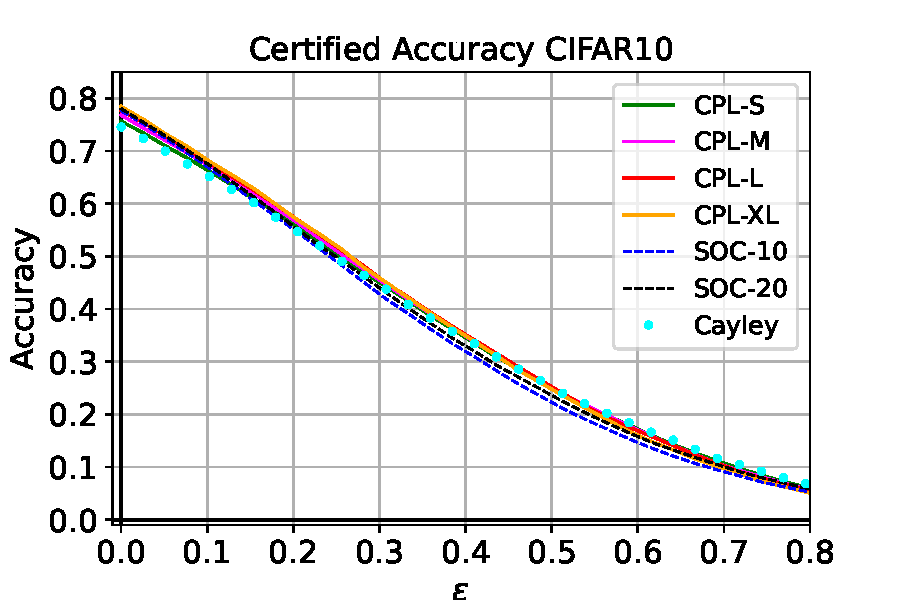
\includegraphics[width =0.48\textwidth]{sections/4_certification/images/cert_acc_eps_c10.pdf} & 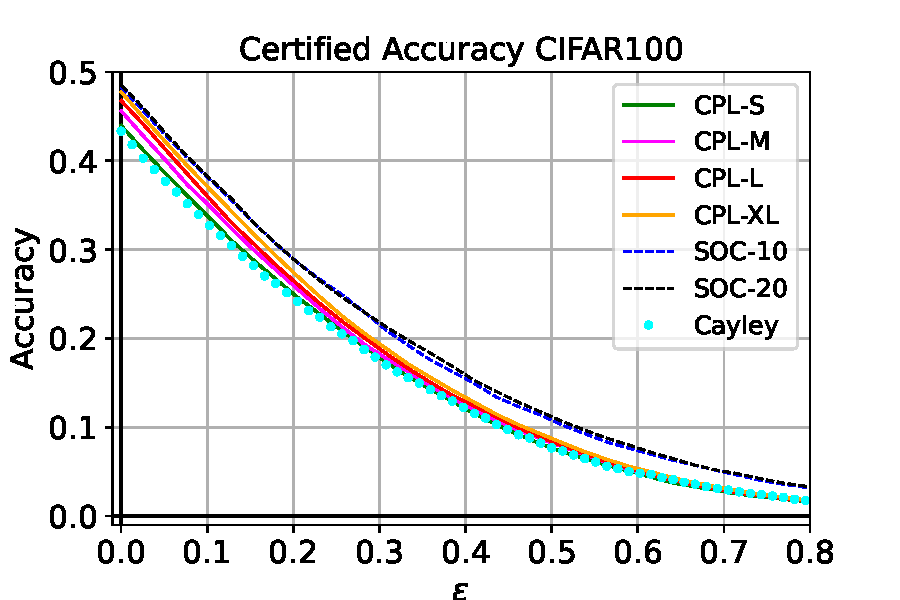
\includegraphics[width =0.48\textwidth]{sections/4_certification/images/cert_acc_eps_c100.pdf}
    \end{tabular}
    \caption{Certifiably robust accuracy in function of the perturbation $\varepsilon$ for our CPL networks and its concurrent approaches (SOC and Cayley models) on CIFAR10 and CIFAR100 datasets.}
    \label{fig:cert-acc}
\end{figure}

\paragraph{Certified Adversarial Robustness.} 
Results on CIFAR10 and CIFAR100 dataset are reported respectively in Tables~\ref{table:c10-comp} and~\ref{table:c100-comp}. We also plotted certified accuracy in function of $\varepsilon$ on Figure~\ref{fig:cert-acc}. On CIFAR10, our method outperforms the concurrent approaches in terms of standard and certified accuracies for every level of $\varepsilon$ except SOC+ that uses additional tricks we did not use. On CIFAR100, our method performs slightly under the SOC networks but better than Cayley networks. Overall, our methods reach competitive results with SOC and Cayley layers. 

Note that we observe a small gain using larger and deeper architectures for our models. This gain is less important as $\varepsilon$ increases but the gain is non negligible for standard accuracies. In term of training time, our small architecture (CPL-S) trains very fast compared to other methods, while larger ones are longer to train.


\begin{figure}[h]
    \centering
    \begin{tabular}{cc}
    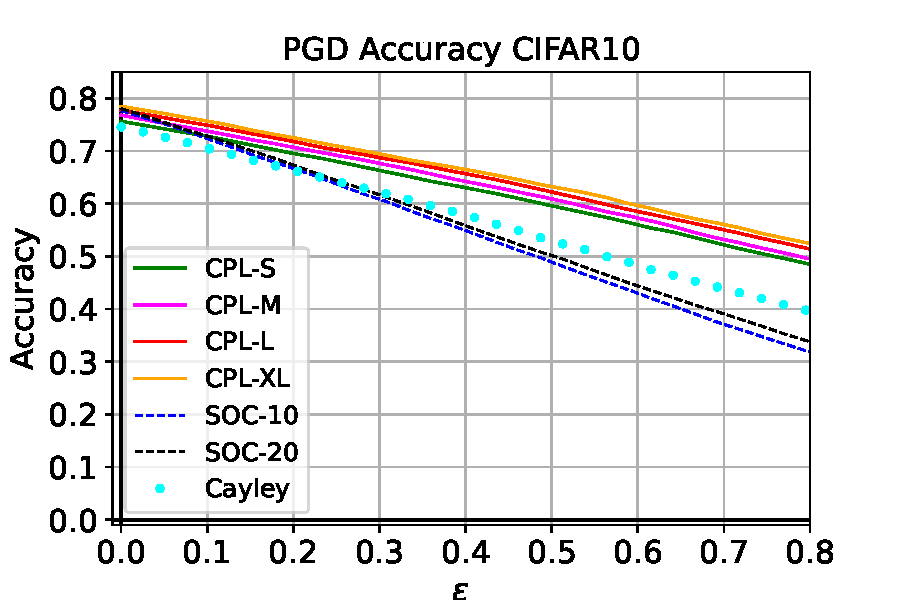
\includegraphics[width =0.48\textwidth]{sections/4_certification/images/pgd_acc_eps_c10.pdf} & 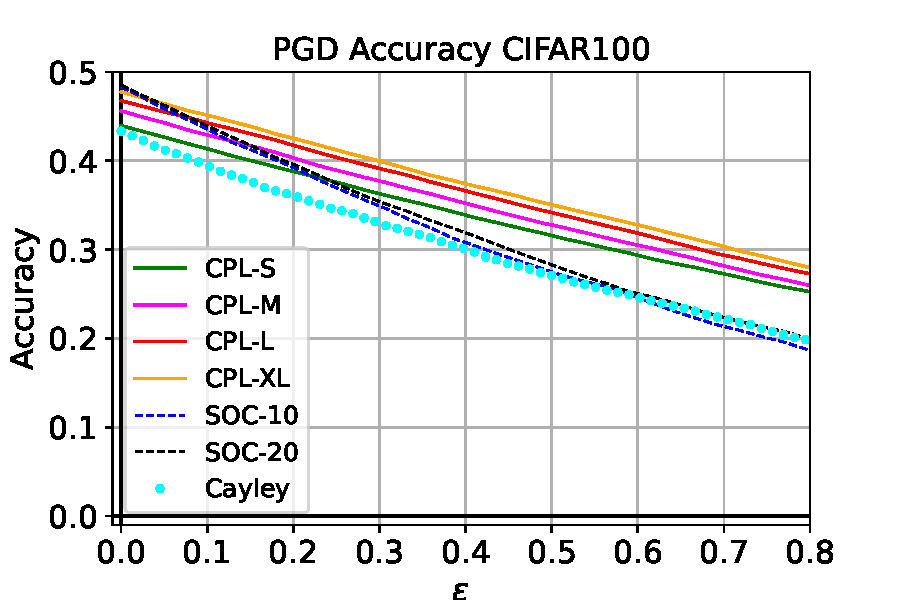
\includegraphics[width =0.48\textwidth]{sections/4_certification/images/pgd_acc_eps_c100.pdf}
    \end{tabular}
    \caption{Accuracy against PGD attack with 10 iterations in function of the perturbation $\varepsilon$ for our CPL networks and its concurrent approaches on CIFAR10 and CIFAR100 datasets.}
    \label{fig:pgd-acc}
\end{figure}
\paragraph{Empirical Adversarial Robustness.} We also reported in Figure~\ref{fig:pgd-acc} the accuracy of all the models against PGD $\ell_2$-attack~\citep{kurakin2016adversarial,madry2017towards} for various levels of $\epsilon$. We used $10$ iterations for this attack. We remark here that our methods brings a large gain of robust accuracy over all other methods. On CIFAR10 for $\varepsilon = 0.8$, the gain of CPL-S over SOC-10 approach is more than $10\%$. For CIFAR100, the gain is about $10\%$ too for $\varepsilon=0.6$. We remark that using larger architectures lead in a more substantial gain in empirical robustness. 

Our layers  only provide an upper bound on the Lipschitz constant, while orthonormal layers as Cayley and SOC are built to exactly preserve the norms. This might negatively influence the certified accuracy since the effective Lipschitz constant is smaller than the theoretical one, hence leading to suboptimal certificates. This might explain why our method performs so well of empirical robustness task.

